\documentclass[a4,center,fleqn]{NAR}

% Enter dates of publication
\copyrightyear{2008}
\pubdate{31 July 2009}
\pubyear{2013}
\jvolume{37}
\jissue{12}

%\articlesubtype{This is the article type (optional)}

\begin{document}

\title{TagDust version 2.0 - a program to extract, filter and correctly label next generation sequencing reads.}

\author{%
Timo Lassmann\,$^{1}$%
\footnote{To whom correspondence should be addressed.
Tel: +44 000 0000000; Fax: +44 000 0000000; Email: xxx@yyyy.ac.zz}}

\address{%
$^{1}$Division of Genomic Technologies, Center for Life Science Technologies,
RIKEN Yokohama Institute,
1-7-22 Suehiro-cho, Tsurumi-ku, Yokohama
230-0045 Kanagawa, Japan 
}
% Affiliation must include:
% Department name, institution name, full road and district address,
% state, Zip or postal code, country

\history{%
Received January 1, 2013;
Revised February 1, 2013;
Accepted March 1, 2013}

\maketitle

\begin{abstract}

Arguably the most basic step in the analysis of next generation sequences (NGS) involves extracting mappable reads from the raw reads produced by the various sequencing instruments. The presence of indices, fingerprints, adaptors and artifacts all of which containing sequencing errors makes this step non-trivial. 

Tagdust2 is designed to carry out all steps required to go from raw- to mappable reads. This includes de-multiplexing libraries, removing adaptors, identifying unique molecular identifiers and discarding artifacts. Our method allows users to specify the expected architecture of a read and converts it into a hidden Markov model (HMM). The latter recognized different segments in the raw reads and assigns reads to a particular barcode even in the presence of sequencing errors. Artifactual sequences, which by definition do not not match the architecture are automatically discarded.

\end{abstract}

\section{Introduction}

Next generation sequencing has greatly accelerated the accumulation of genomics data. Different protocols targeting the genome, epi-genome and transcriptions are widely used\cite{ENCODEINTEGRATION}. In essence, all protocols capture biological sequences of interest while adding adaptors and other sequences to facilitate cost effective sequencing. An obvious examples here is the use of indices or barcodes allowing researchers to profile multiple samples in a single lane\cite{Craig:2008,Kircher:2012}. In addition recent protocols have added stretches of random sequences in order to correct for PCR and other biases \cite{Kivioja:2012kg}. In summary, the number of nucleotides used to describe what is being sequenced is increasing. As the length increases so is the chance that sequencing errors occur in these key sequences. In the best case these errors lead to some sequences being lost to the downstream analysis, but in the worse case sequences can be mixed up between samples leading to analytical noise.

Sequencers have different error rates.

We previously released TagDust to remove artifactual reads\cite{Tagdust2009}. While being useful, the focus on identifying and discarding whole reads meant that most processing pipelines using TagDust required many additional programs and steps. Here I describe TagDust2 a program designed to carry out all steps required to go from raw reads to sequences ready to be mapped. The key part of finding the mappable read and annotating it based on barcodes is carried out by a user defined hidden Markov model.(HMM). problem here is quite similar to many problems in biological sequence analysis: identifying domains TMM segments etc. Therefore I decided to approach this problem as a sequence labeling problem for which hidden Markov models (HMMs) are suitable. 

 
% **************************************************************
% Keep this command to avoid text of first page running into the
% first page footnotes
\enlargethispage{-65.1pt}
% **************************************************************
\section{MATERIALS AND METHODS}

\subsection{General Approach}

\begin{figure}[t]
\begin{center}
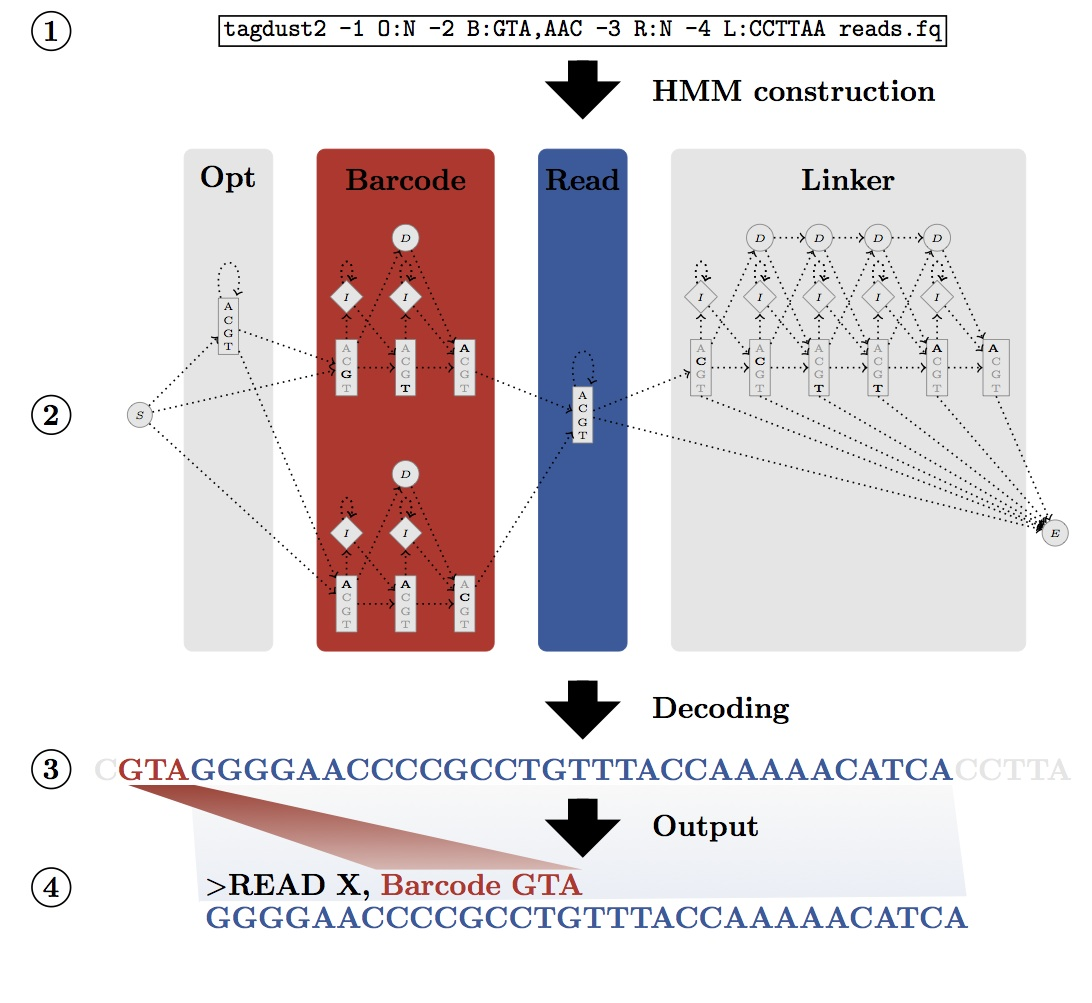
\includegraphics[scale = 0.5]{../figures/figure1.pdf}
\end{center}
\caption{Overview of the TagDust workflow. Sequences are labelled according to the HMM architecture and relevant information written to the output. 
}
\label{figure1}
\end{figure}

TagDust implements a small library of HMMs which I will refer to as segments. Each segment contains a silent start and end state which are used to connect multiple segments. Segments are hand-designed to capture commonly occurring features in raw sequences such as the combination of barcodes, variable length sequences and so on. For a complete list see table 1. Users can use a simple command line interface to specify the expected sequence of segments in their reads. TagDust automatically constructs a global HMMs from the segments and starts scoring the individual reads (see Figure \ref{figure1}). 

Parameterization... 

\subsection{Sequence scoring} 

TagDust implements the basic forward and backward algorithm as described in \citep{durbin}. For each sequence the logs odds score is defined by the summed probability of all paths (forward score) divided by the probability of a background zero order Markov model. The latter is parameterized based on the length and nucleotide distribution in the input reads. 

\begin{equation}
	S  = log \left(  \frac{P(M)}{P(R)} \right) + log \left(\frac{\sum\limits_{\pi} P(x,\pi | M )}{P(x | R ) } \right)
\end{equation}

The prior probabilities $P(M)$ and  $P(R)$ are set to 0.9 and 0.1 respectively. Finally, the log odds score is converted into a probability using the logistic function:

\begin{equation}
	P(M | x) = \frac{e^S}{1-e^S}
\end{equation}

If barcodes are present TagDust calculated an additional confidence score. At every building block containing multiple transitions from the silent state to HMMs, TagDust calculates the maximum probability of selecting one particular transition:       


\begin{equation}
	V = \max_j \left( \frac{f_s(i)  ( a_{s,m_j} e_{m_j}(x+1) b_{m_j}(i+1)+  a_{s,I_j} e_{I_j}(x+1) b_{I_j}(i+1))}{\sum\limits_{\pi} P(x,\pi | M )}\right)
\end{equation}

where $m_j$ and $I$ are the first match and insert states of a barcode HMM model. In essence this probability reflects how confident we are in selecting one barcode over any other. 

As a default TagDust only extracts reads if $V$ is greater than 0.5 and $P(M | x)$ is greater than 0.99. 

\subsection{Optimal accuracy decoding} 

To obtain the most probable labeling of the sequence, I employ the optimal accuracy decoding algorithm as described in \citep{Kall:2005vg}. To apply this algorithm to our problem define the label probability of a nucleotide by the summed posterior label probabilities of all states belonging to a particular HMM segment. A secondary dynamic programming algorithm is used to determine the path with the maximal label probability, constrained by the global HMM architecture. The label probabilities are essentially used as a substitution matrix while the architecture is enforced by the equivalent of gap penalties. 

If fingerprints are present TagDust checks at this stage if the length after decoding matches the users input. If not the read is discarded. 

\subsection{Implementation} 

Internally, TagDust uses full profile HMMs for each segment. To emulate different segments we simply set some transition probabilities to zero. For example the read building block 'R' is implemented as a profile HMM with one column and transitions directly to and from the insertion state. We parallelized the most computationally demanding parts using threads. TagDust is written in C and the source code is freely available here: 



\subsection{Further read filtering}

TagDust allows users to specify a fasta file containing known sequences the user wishes to exclude from mapping. For example in transcriptome sequencing one commonly wants to remove ribosomal sequences from the downstream analysis. To address this issue in a general manner Tagdust exhaustively align all reads to the target reference sequences and discard all reads with less than X mismatches. For efficiency we implemented the Myers bit parallel algorithm\cite{MyersDYN} using SIMD instructions as well as using thread level parallelism. 

\subsection{Filtering low complexity sequences.}
Tagdust implements a simplified version of the DUST module (R. Tatusov and D.J. Lipman, unpublished data) to filter out low complexity reads. While this is not strictly necessary for NGS reads I implemented it to remove poly-A and other "very" low complexity sequences. The algorithm is only applied to the first sixty-four nucleotides of the reads. 





\section{RESULTS}

\subsection{Large benchmark}

To assess the accuracy of TagDust in a wide range of possible applications, we simulate datasets containing barcodes of different length and varying sequencer error rates. In all experiments we simulated 900k barcode containing sequences and 100k random sequences which should not be extracted. We compared our results to the program fastx barcode splitter from the fastX package. This program allows for sequencing errors in the barcodes and performs much better than approaches using exact pattern matching. 

In all our simulated test cases, TagDust mis-aligns less than half a percent of the reads to the wrong library. As expected, in noisy datasets fewer reads are extracted. In contrast, this percentage is usually higher in fastx. In addition, the simple strategy using one mismatch leads fastx to assign between 25 - 100\% of the random sequences to a library. Using default parameters, Tagdust does not extract any reads when using many short barcodes. 

\begin{figure*}[t]
\begin{center}
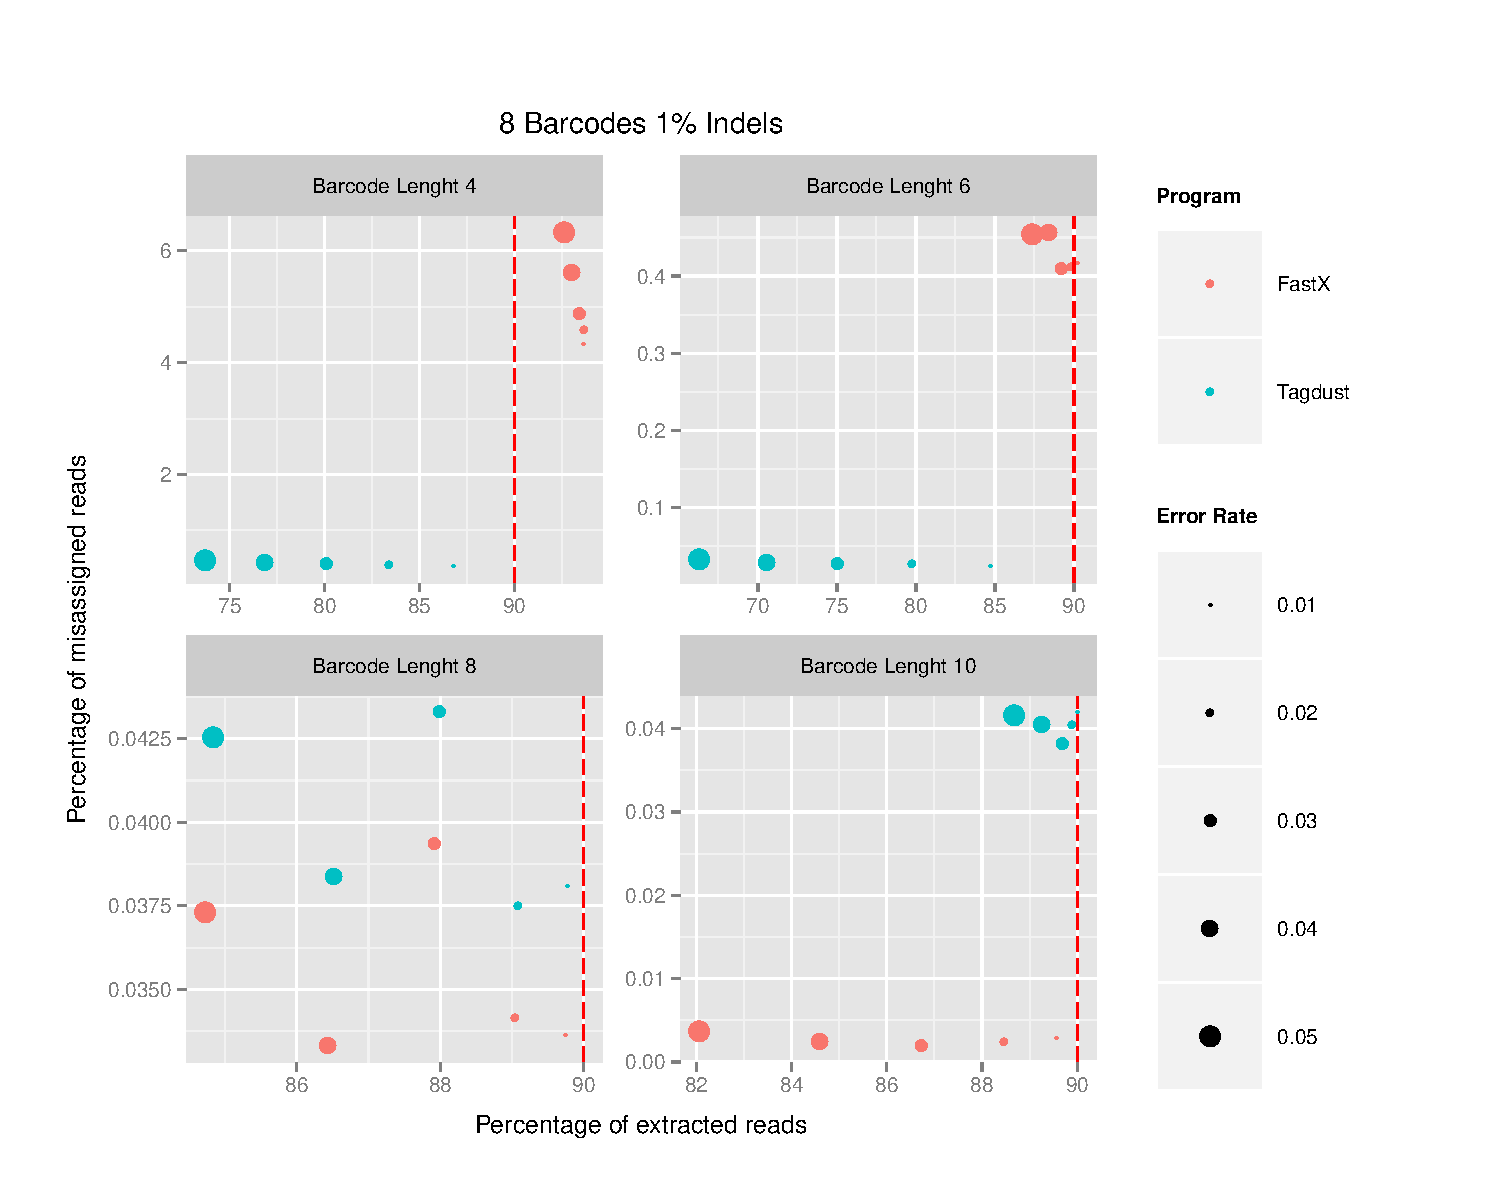
\includegraphics[scale = 0.2]{../figures/8Barcodes1Indels.pdf}
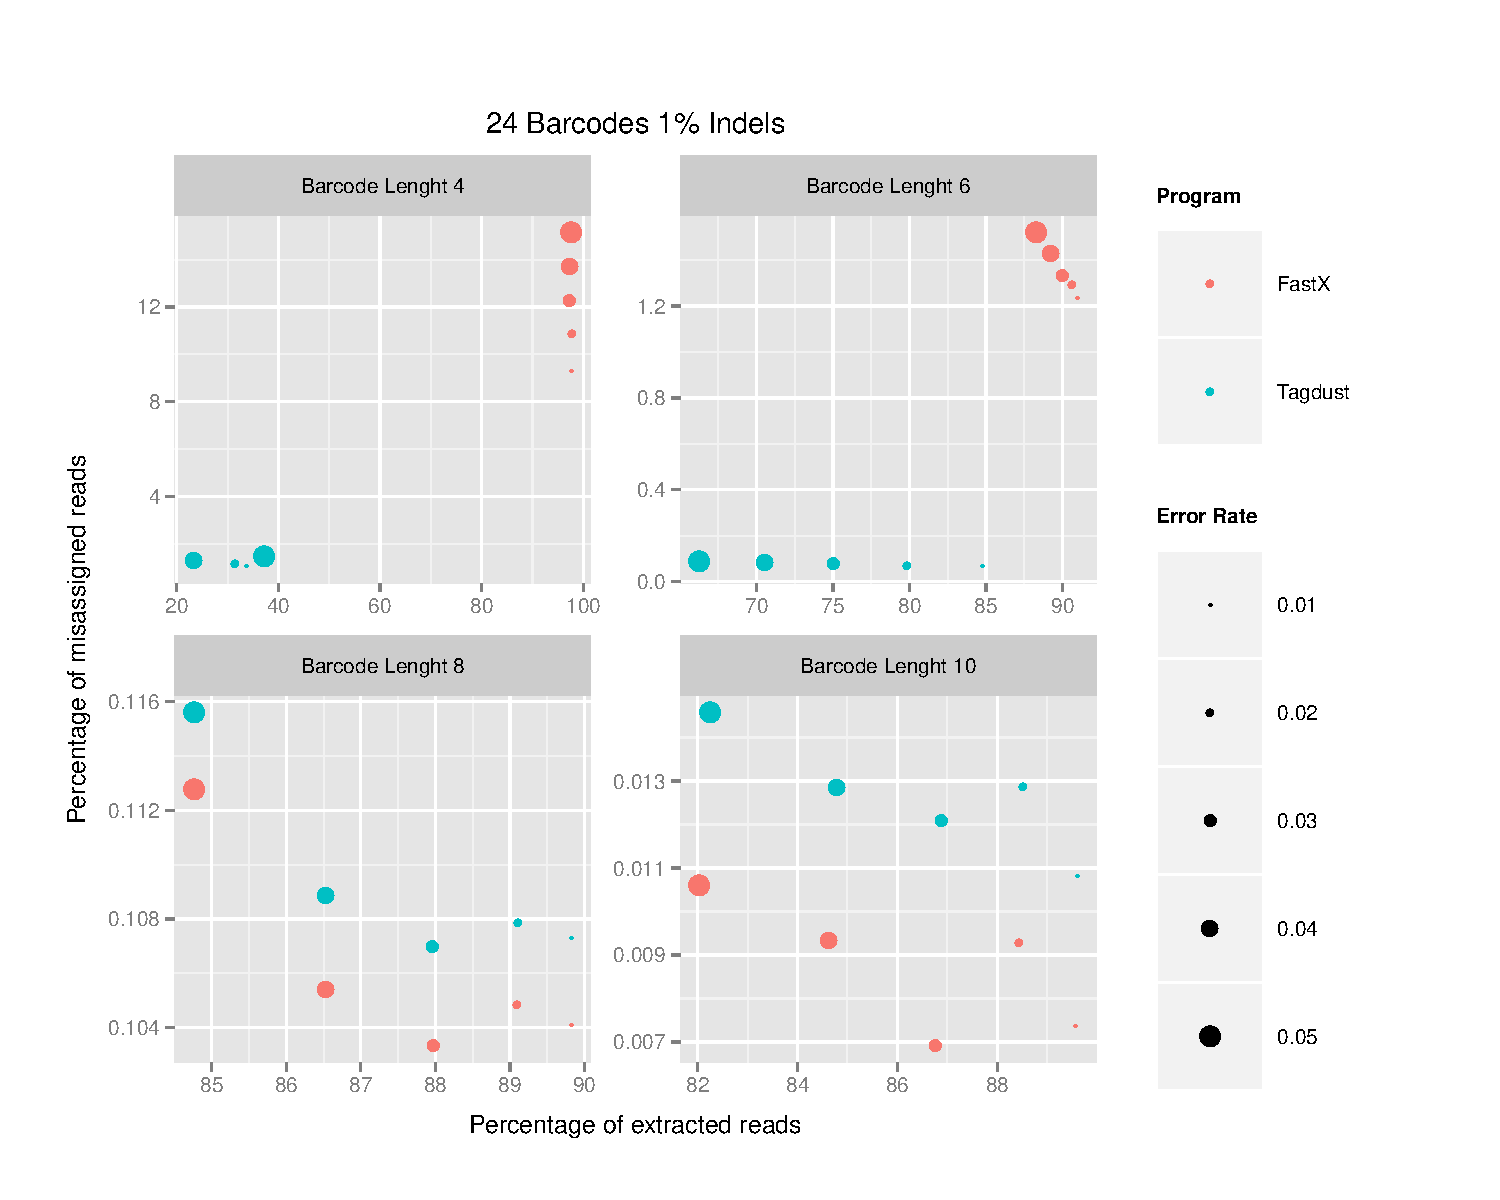
\includegraphics[scale = 0.2]{../figures/24Barcodes1Indels.pdf}
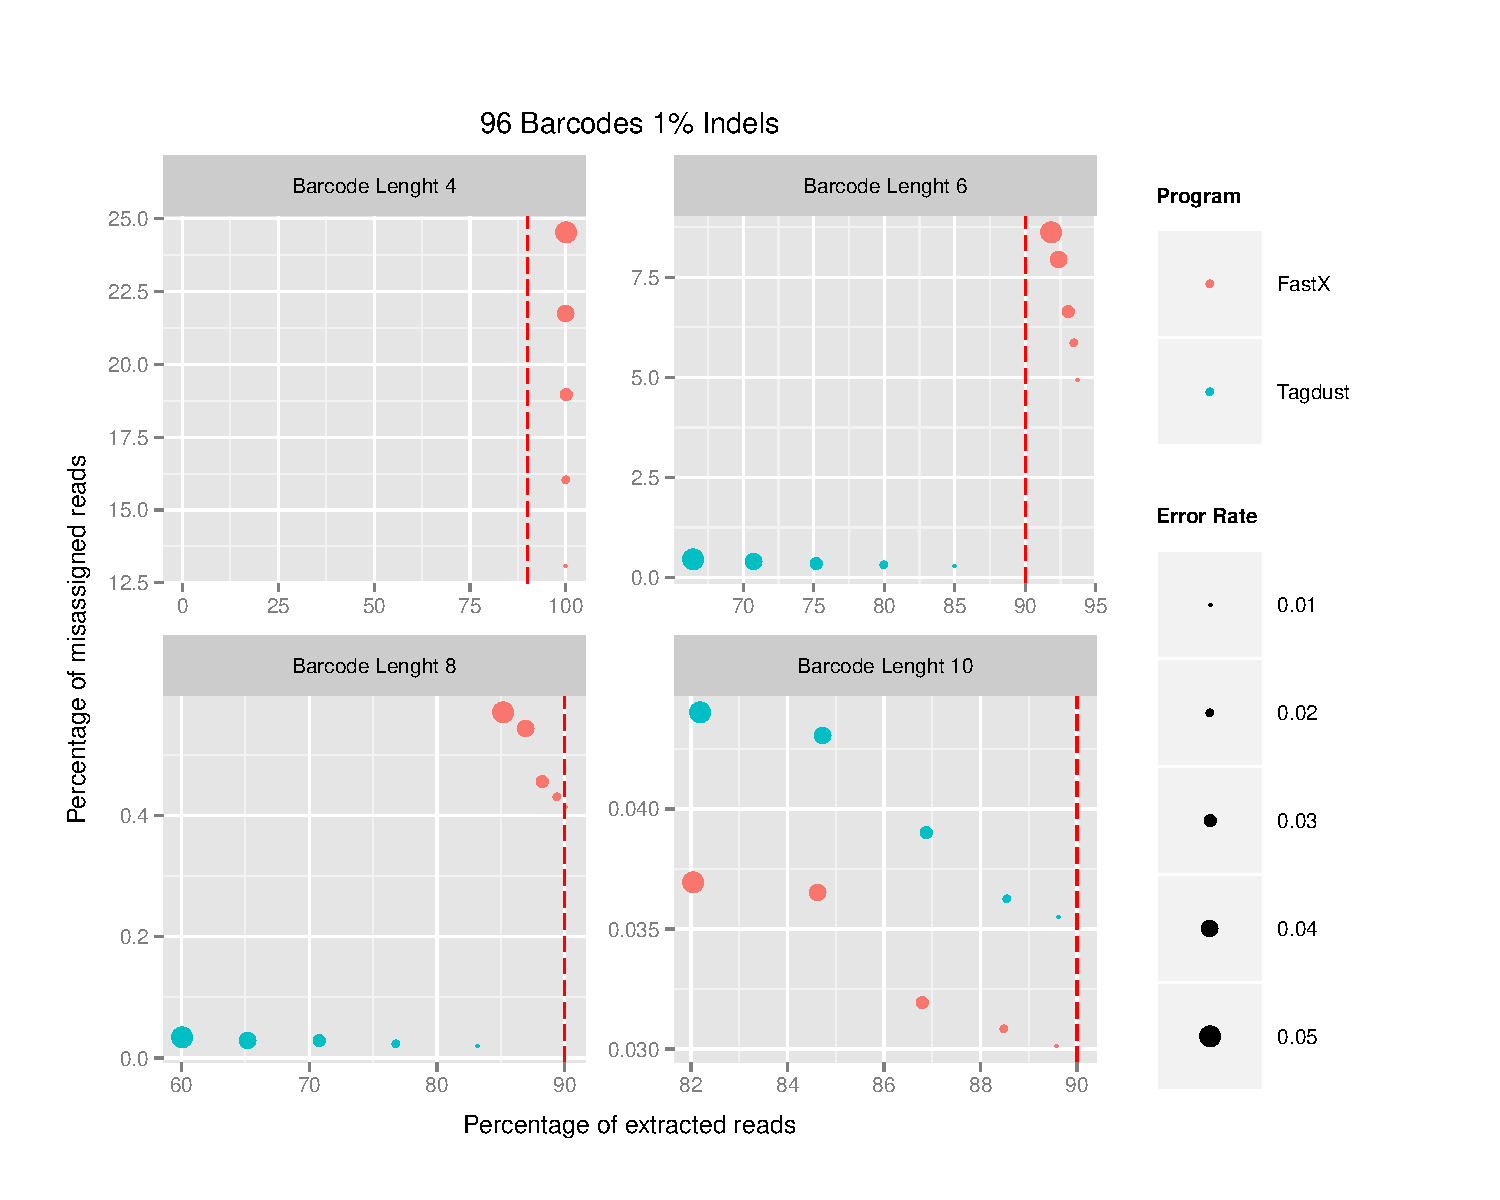
\includegraphics[scale = 0.2]{../figures/96Barcodes1Indels.pdf}
\end{center}
\caption{Performance of TagDust and Fastx at extracting reads containing 8 \textbf{(left)} and 96 \textbf{(right)} different barcodes. Different barcode lengths are shown in the different panels. The size of each datapoint represents the error rate ranging from 1 - 5\%. The read line indicates the maximum number of reads that should be extracted.
}
\label{figure2}
\end{figure*}

\subsection{Extraction rate on read data.}



\begin{table}[b]
\tableparts{%
\caption{Summary of single cell extracted reads.}
\label{table:01}%
}{%
\begin{tabular*}{\columnwidth}{@{}lrr@{}}
\toprule
Description & Number of Reads & Percentage
\\
\colrule
Total reads   & 110622138 & 100.00\%\\
\colrule
Problems with architecture & 8503361 & 7.69\%\\
Low Complexity & 7228724 & 6.53\%\\
Ambiguous barcode & 59574  &0.05\% \\
Too short & 1  & 0.00\%\\ 
\colrule
Extracted & 94830478 & 85.72\%\\
\botrule
\end{tabular*}%
}
{This is a table footnote}
\end{table}
7.69%
6.53%
0.05%
85.72%



\begin{table}[b]
\tableparts{%
\caption{Summary of UMI extracted reads.}
\label{table:01}%
}{%
\begin{tabular*}{\columnwidth}{@{}lrr@{}}
\toprule
Description & Number of Extracted Reads & Percentage
\\
\colrule
15 PCR cyles & 62110757 & 96.0\%\\
25 PCR cyles & 75824331 & 95.1\%\\
\colrule
1000 cells & 87271807 & 95.8\%\\
100 cells & 58146883  & 87.8\% \\
10 cells & 27051690  & 67.2\%\\ 
\botrule
\end{tabular*}%
}
{This is a table footnote}
\end{table}






\begin{figure}[t]
\begin{center}
\includegraphics[scale = 0.5]{../figures/comp_15c_repeat1_25c_repeat1_umi.pdf}
\includegraphics[scale = 0.5]{../figures/comp_15c_repeat1_25c_repeat1_noumi.pdf}
\end{center}
\caption{Caption for wide figure over two columns.
\textbf{(a)} Left figure.
\textbf{(b)} Right figure (see (a)).
}
\label{NAR-fig2}
\end{figure}


\subsection{Results subsection three}



\section{DISCUSSION}

\subsection{Discussion subsection one}

Text. Text. Text. Text. Text. Text. Text. Text. Text. Text. Text.
Text. Text. Text. Text. Text. Text. Text. Text. Text. Text. Text.
Text. Text. Text. Text. Text. Text. Text. Text. Text. Text. Text.
Text. Text. Text. Text. Text. Text. Text. Text. Text. Text. Text.


\subsection{Discussion subsection two}

Text. Text. Text. Text. Text. Text. Text. Text. Text. Text. Text.
Text. Text. Text. Text. Text. Text. Text. Text. Text. Text. Text.
Text. Text. Text. Text. Text. Text. Text. Text. Text. Text. Text.
Text. Text. Text. Text. Text. Text. Text. Text. Text. Text. Text.
Text. Text. Text. Text. Text. Text. Text. Text. Text. Text. Text.
Text. Text. Text. Text. Text. Text. Text. Text. Text. Text. Text.
Text. Text. Text. Text. Text. Text. Text. Text. Text. Text. Text.
Text. Text. Text. Text. Text. Text. Text. Text. Text. Text. Text.
Text. Text. Text. Text. Text. Text. Text. Text. Text. Text. Text.
Text. Text. Text. Text. Text. Text. Text. Text. Text. Text. Text.
Text.



%\begin{figure}[t]
%\begin{center}
%\includegraphics{NAR-fig1.eps}
%\end{center}
%\caption{Caption for figure within column.}
%\label{NAR-fig1}
%\end{figure}

\subsection{Discussion subsection three}

Tagdust2 is both accurate and versitile. 
Text. text. 
Compared to other is wins. 

\section{CONCLUSION}

As wet protocols become more sophisticated and take full advantage of longer read lengths the architecture of raw reads is becoming ever more complex. Tagdust2 can be used to correctly annotate reads in one step. 

The present version requires users to specify the expected error frequency of the sequencer. In future I plan to estimate these parameters directly for ever segment using simple learning from labelled sequences. Quality values... .


In future we may consider learning the architecture from the sequencing data directly. However, at the moment investigators usually know what should be there and wherer. 




\section{ACKNOWLEDGEMENTS}
This work was supported by a Research Grant from the Japanese Ministry of Education, Culture, Sports, Science and Technology (MEXT) to the RIKEN Center for Life Science Technologies.

\subsubsection{Conflict of interest statement.} None declared.
\newpage


\begin{thebibliography}{4}

% Format for article

\bibitem{ENCODEINTEGRATION}
Ian Dunham, {\it et. al.} (2012)
An integrated encyclopedia of DNA elements in the human genome.
\textit{Nature}, \textbf{489},57�74.

\bibitem{Craig:2008}
Craig DW, Pearson JV, Szelinger S, Sekar A, Redman M, Corneveaux JJ, Pawlowski TL, Laub T, Nunn G, Stephan DA, \textit{et al.} (2008)
Identification of genetic variants using bar-coded multiplexed sequencing.
\textit{Nat. Methods}, \textbf{5}, 887-893.

\bibitem{Kircher:2012}
Kircher, M., Sawyer, S., and Meyer, M. (2012).
Double indexing overcomes inaccuracies in multiplex sequencing on the Illumina platform.
\textit{Nucleic acids research}, \textbf{40}(1), e3. 

\bibitem{Kivioja:2012kg}
Kivioja, T., V�h�rautio, A., Karlsson, K., Bonke, M., Enge, M., Linnarsson, S., and Taipale, J. (2012).
Counting absolute numbers of molecules using unique molecular identifiers.
\textit{Nature methods}, \textbf{9}(1), 72-74.

\bibitem{Tagdust2009}
Lassmann, T., Hayashizaki, Y., and Daub, C. O. (2009).

TagDust - a program to eliminate artifacts from next generation sequencing data.
\textit{Bioinformatics}, \textbf{25}(21), 2839-2840. 

\bibitem{MyersDYN}
Myers, G. (1999).
A fast bit-vector algorithm for approximate string matching based on dynamic programming.
\textit{Journal of the ACM}, \textbf{46}, 1�13.


% Format for book
\bibitem{2}
Author,D., Author,E.F. and Author,G. (1995)
\textit{Book Title}.
Publisher Name, Publisher Address.

% Format for chapter in book
\bibitem{3}
Author,H. and Author,I. (2005)
Chapter title.
In
Editor,A. and Editor,B. (eds),
\textit{Book Title},
Publisher Name, Publisher Address,
pp.\ 60--80.

% Another article
\bibitem{4}
Author,Y. and Author,Z. (2002)
Article title.
\textit{Abbreviated Journal Name}, \textbf{53}, 500--520.
\bibitem{gaga}
Author,A.B. and Author,C. (1992)
Article title GAGAGAGAGA.
\textit{Abbreviated Journal Name}, \textbf{5}, 300--330.




%@article{Kivioja:2012kg,
%author = {Kivioja, Teemu and V{\"a}h{\"a}rautio, Anna and Karlsson, Kasper and Bonke, Martin and Enge, %Martin and Linnarsson, Sten and Taipale, Jussi},
%title = {{Counting absolute numbers of molecules using unique molecular identifiers.}},
%journal = {Nature methods},
%year = {2012},
%volume = {9},
%number = {1},
%pages = {72--74},
%month = jan
%}


%@book{durbin,
%    author = {Durbin, R. and Eddy, S. and Krogh, A. and Mitchison, G.},
%    edition = {eleventh},
%publisher = {Press, Cambridge U.},
%    title = {{Biological sequence analysis}},
%    year = {2006}
%}



%@article{Kall:2005vg,
%author = {K{\"a}ll, Lukas and Krogh, Anders and Sonnhammer, Erik L L},
%title = {{An HMM posterior decoder for sequence feature prediction that includes homology information}},
%journal = {Bioinformatics (Oxford, England)},
%year = {2005}
%}




\end{thebibliography}

\end{document}
